\documentclass[a4paper]{article}


\usepackage{alphabeta} 
\usepackage{enumitem} 
\usepackage{mathtools}
\usepackage{amsmath, amssymb} 
\usepackage{amsthm}
\usepackage{cancel} 
\usepackage[margin=0.70in]{geometry} 
\geometry{left=3cm,right=3cm,top=2.4cm,bottom=2.8cm}	%the page geometry as defined, A4=210x297mm
\usepackage{graphicx}
\usepackage{wrapfig}
\usepackage{caption}
\usepackage{textcomp}
\usepackage{tabto}
\usepackage{layout}
\usepackage{bm}
\usepackage{minipage-marginpar}
\usepackage[dvipsnames]{xcolor}
\usepackage{hyperref}
\usepackage{dutchcal}
\usepackage{derivative}
\usepackage{esint}
%\usepackage{biblatex}
\usepackage{subcaption}
\usepackage{booktabs}\usepackage{derivative}
\usepackage[flushleft]{threeparttable}
\usepackage[capbesideposition=outside,capbesidesep=quad]{floatrow}


%%RENEW

\newtheorem{problem}{Άσκηση}
\newtheorem*{solution*}{Λύση}
\newtheorem{definition}{Ορισμός}[subsection]
\newtheorem{properties}{Ιδιότητες}[subsection]
\newtheorem{theorem}{Θεώρημα}[subsection]
\newtheorem{protash}{Πρόταση}[subsection]
\newtheorem{porisma}{Πόρισμα}[subsection]
\newtheorem{lemma}{Λήμμα}[subsection]
\newtheorem*{prooof}{Απόδειξη}
\newtheorem*{notes}{Παρατηρήσεις}
\newtheorem*{note}{Παρατήρηση}
\newtheorem*{app}{Εφαρμογή} 
\newtheorem*{example}{Παράδειγμα}
\newtheorem*{examples}{Παραδείγματα}

%\renewcommand{\labelenumi}{\roman{enumi}}
\newcommand{\approxtext}[1]{\ensuremath{\stackrel{\text{#1}}{\approx}}}
\renewcommand{\figurename}{Εικόνα.}
\renewcommand{\tablename}{Πίνακας.}
%\renewcommand\refname{New References Header}
\renewcommand*\contentsname{Περιεχόμενα}

\begin{document}
\begin{titlepage}			%makes a title page. Remember to change the author, CID, username and group number to what is appropriate for you!
	\centering
	{\scshape\LARGE Εθινικό Μετσόβιο Πολυτεχνείο\par}
	{\scshape \LARGE Σ.Ε.Μ.Φ.Ε.\par}
	\vspace{1cm}
	{\huge\bfseries Μελέτη Ακουστικών Κυμάτων σε Ηχητικό Σωλήνα\par}
	\vspace{1cm}
	{\Large\itshape Θωμόπουλος Σπύρος\par}		%remember to change these!
	
	%		{\large Group \@group\unskip\strut\par}
	{\large A.M ge19042 \hfill \\}% spyros.thomop@gmail.com/ ge19042@mail.ntua.gr\par		%remember to change these!
	\vspace{1cm}
	{\large 29 /10/2021\par}
\end{titlepage}


\newpage 


\section*{Σκοπός}
Ο στόχος της εν λόγω πειραματικής άσκησης είναι να μελετηθούν τα στάσιμα ακουστικά κύματα στον αέρα εντός ηχητικού σωλήνα με κλειστά άκρα και με ανοικτό-κλειστό άκρο. Συγκεκριμένα θα ασχοληθούμε με το κύμα της ακουστικής πίεσης για τις πρώτες δύο συχνότητες συντονισμού. Ακόμη, θα προσδιορισθεί η ταχύτητα διάδοσης του ήχου με την μέθοδο των στασίμων κυμάτων και με την μέθοδο radar.

\section*{Θεωρητικά Στοιχεία}
\subsubsection*{Περί Ηχητικού Κύματος}
Ο ήχος είναι ένα διάμηκες κύμα. Κύμα, διότι πρόκειται για ταλαντωτικές διακυμάνσεις στην πίεση/πυκνότητα και για μικρές ταλαντώσεις των μορίων του αέρα, ενώ διάμηκες διότι οι παραπάνω κινήσεις συμβαίνουν κάθετα στην διεύθυνση διάδοσής του. 
%Η έναρξη της διάδοσης συμβαίνει με την ταλάντωση στερεών (π.χ. μεμβρανών) τα οποία βρίσκονται σε επαφή με τον αέρα.
Η διατάρραξη των μορίων σε κάποιο σημείο του αέρα από την Θέσση Ισορροπίας τους προκαλείται από αλληλεπιδράσεις με άλλα μόρια τα οποία βρίσκονται σε περιοχές απ' όπου προέρχεται το κύμα. Αυτή η λογική συνεπάγεται πως υπάρχει ένα σημείο ή μία περιοχή του χώρου στην οποία δημιοργούνται τα ηχητικά κύματα, η πηγή. Η πηγή μπορεί να είναι κάποιο στερεό αντικείμενο εντός του αέρα (π.χ. μεμβράνη) το οποίο ταλαντώνεται περιοδικά με μία συχνότητα, η οποία είναι και η συχνότητα του κύματος. 

%Η σύνδεση των παραπάνω με την διακύμανση της πυκνότητας είναι η εξής: 

Η περιοδική κίνηση των μορίων σχετίζεται άμεσα με την περιοδική διακύμανση της πίσεσης/πυκνότητας του αέρα. Αν η πηγή ξεκινήσει την ταλάντωσή της προς την διεύθυνσης διάδοσης του κύματος, τότε υπάρχει μία περιοχή όπου συνωστίζονται τα μόρια, άρα εκεί αυξάνεται η πυκνότητα και η πίεση (πύκνωμα). Όταν η πηγή ξεκινήσει την αντίθετη κίνησή της δημιοργείται περιοχή χαμηλής πυκνότητας άρα και πίεσης (αραίωμα), η οποία καταλαμβάνεται από ένα μέρος των μορίων του πυκνώματος. Το υπόλοιπο μέρος κινείται προς την διεύθυνση διάδοσης παρασέρνωντας τα επόμενα μόρια σε κίνηση και πλέον το αρχικό πύκνωμα μετατρέπεται σε αραίωμα. Τα βήματα αυτά επαναλαμβάνονται και έτσι διαδίδεται το ακουστικό κύμα. 

Υπάρχει και η περίπτωση η έναρξη της διαδικασίας να συμβαίνει με την πηγή να κινείται αντίθετα από την διεύθυνση διάδοσης με αποτέλεσμα απλώς η πρώτη διαταραχή να είναι αραίωμα.


\subsubsection*{Περί Στάσιμου ηχητικού κύματος}
Όταν δύο αντίθετα διαδιόμενα ηχητικά κύματα ίδιας συχνότητας (f) και ίδου πλάτους $y_0$, που προκαλούν κύματα πίεσης πλάτους $p_0$, συμβάλλουν στον ίδιο περιορισμένο χώρο δημιουργούνται στάσιμα ακουστικά κύματα. Σε αυτά, το κάθε σημείο του μέσου έχει συγκεκριμένο πλάτος ταλάντωσης το οποίο εξαρτάται από τις συνοριακές συνθήκες γεγονός που διαφαίνεται από την εξίσωση στάσιμου κύματος για την μετατόπιση: 
\begin{equation}\label{1}
y_x  =  2y_0 sin(\frac{2\pi}{\lambda}x)cos(\omega t+\alpha) 
\end{equation}

Στην περίπτωσή μας τα κύματα συμβάλλουν εντός ενός κυλινδρικού ακουστικού σωλήνα. Οι πιθανές συνοριακές συνθήκες για τα άκρα του σωλήνα είναι 1) Κλειστό-Κλειστό, 2) Κλειστό-Ανοικτό και 3) Ανοικτό-Ανοικτό. Εμείς, επειδή στο ένα άκρο τοποθετούμε την πηγή μας, δηλαδή θα είναι πάντα κλειστό θα μελετήσουμε μόνο τις πρώτες δύο περιπτώσεις.

Υφίστανται ορισμένα σημεία τα οποία είναι πάντοτε ακίνητα, οι \textit{δεσμοί}, με την απόσταση δύο διδοχικών δεσμών να είναι $\lambda/2$ όπως προκύπτει από την εξίσωση (\ref{1}) αν θέσουμε $y_x=0$. Εκεί, λόγω υψηλής συσσώρευσης των μορίων, η πυκνότητα και η πίεση παιρνουν τη μέγιστη τιμή τους και λέμε πως έχουμε \textit{κοιλίες} πίεσης. Αντίθετα, τα σημεία με την μέγιστη μετατόπιση καλούνται \textit{κοιλίες} μετατόπισης και ταυτίζονται χωρικά με τους \textit{δεσμούς} πίεσης. Προκύπτει απ' την (\ref{1}), πως η απόσταση δεσμού-κοιλάς μετατόπισης είναι $\lambda/4$. Εφόσον ο δεσμός μετατόπισης ταυτίζεται χωρικά με την κοιλία πίεσης, η χωρική διαφορά διαδοχικών δεσμών μετατόπισης και πίεσης είναι $\lambda/4$ που μεταφράζεται σε διαφορά φάσης $\pi/2$. Συνεπώς η εξίσωση πίεσης είναι: 
\begin{equation}\label{2}
y_p  =  2p_0 sin(\frac{2\pi}{\lambda}x)sin(\omega t+\alpha) 
\end{equation}
\textit{Εφαρμογή των Συνοριακών Συνθηκών}\\

a) Κλειστά και τα δύο άκρα. Τότε είναι προφανές πως στα άκρα έχουμε δεσμούς μετατόπισης, άρα κοιλές πίεσης. Στην (\ref{1}), παγώνοντας τον χρόνο, θέτουμε $y_x(0)=y_x(L_a)=0$ και προκύπτει πως το κύμα λαμβάνει συγκεκριμένες τιμές μήκους κύματος που δίνονται απ' τη σχέση 
\begin{equation}\label{3}
\lambda_n = \frac{2L_a}{n}
\end{equation}
όπου $L_a$ είναι το ακουστικό μήκος του σωλήνα το οποίο σε αυτή τη περίπτωση ισούται με το γεωμετρικό μήκος, L, διότι τα άκρα είναι κλειστά. \\ 

b) Ένα ανοικτό και ένα κλειστό άκρο. Εδώ έχουμε δεσμό μετατόπισης/κοιλία πίεσης στο κλειστό άκρο και κοιλία μετατόπισης/δεσμό πίεσης στο ανοικτό άκρο. Ξανά στην ($\ref{1})$, παγώνοντας τον χρόνο, εφάρμόζομυε τις συνοριακές $y_x(0)= 0\Rightarrow \alpha =0$ και  $y_x(L_a)=2y_0$ απ' την οποία προκύπτει
\begin{equation}\label{4}
\lambda_n = \frac{4L_a}{n}
\end{equation}
όπου σε αυτή τη περίπτωση το ακουστικό μήκος είναι $L_a = L+0.63R$.
\\ 
%Αν Q είναι ο συντελεστής ποιότητας του ταλαντωτή-στήλη αέρα, τότε υπάρχουν ορισμένες συχνότητες διέγερσης για τις οποίες επιτυγχάνεται συντονισμός που σημαίνει μεγιστοποίηση, δηλαδή η αύξηση κατά Q φορές, των παραμέτρων της ταλάντωσης όπως η μετατόπιση των μορίων καιη πίεση της αέριας στήλης.

%Στην διάταξή μας η πηγή των κυμάτων είναι ένα μεγάφωνο που τοποθετείεται στο ένα άκρο
Οι συχνότητες κύματος που αντιστοιχούν στα μήκη κύματων των εξισώσεων (\ref{3}) και (\ref{4}) καλούνται συχνότητες συντονισμού ή αρμονικές συχνότητες.


\section*{Πειραματική Διάταξη}
Η πειραματική διάταξη αποτελείται από:
\begin{itemize}
\item[.] Μεγάφωνο που χρησιμεύει ως πηγή ακουστικών κυμάτων
\item[.] Γεννήτρια παλμών για να τροφοδοτεί το μεγάφωνο
\item[.] Ηχητικός σωλήνας από πλεξιγκλάς μήκους $L=90cm$, εσωτερικής ακτίνας $r=1.6cm$ με ενσωματωμένο υποδεκάμετρο
\item[.] Μικρόφωνο για μετατροπή της πίεσης της αέριας στήλης σε ηλετρικό σήμα
\item[.] Ενισχυτή για την ενίσχυση του σήματος του μικροφώνου
\item[.] Παλμογράφο 2 καναλιών για την καταγραφή του σήματος
\end{itemize}

\begin{figure}[h!]
\centering
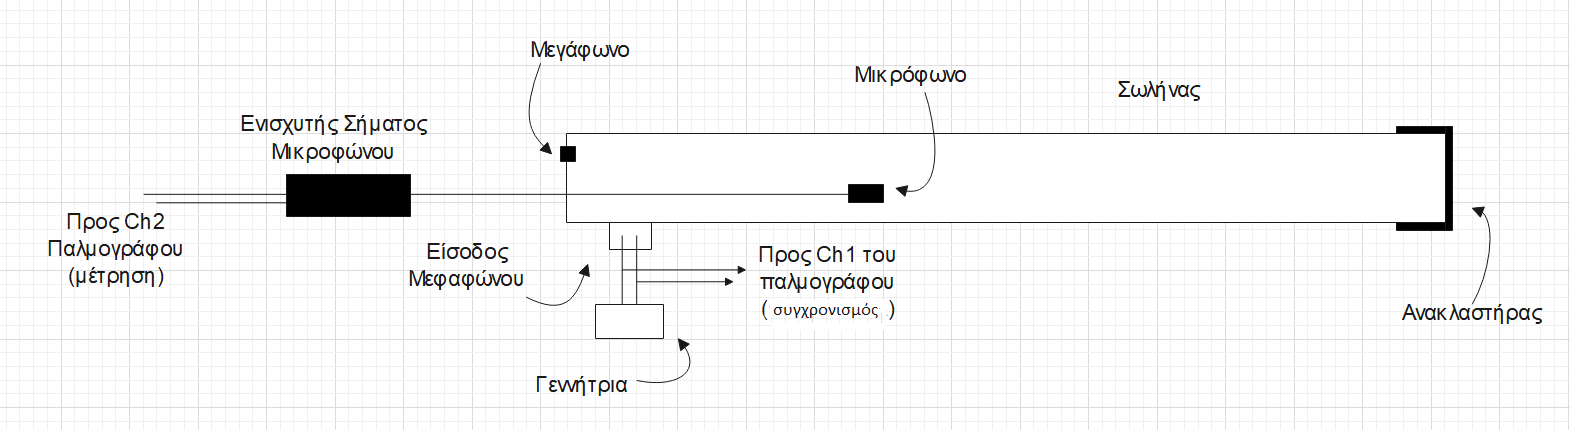
\includegraphics[scale=0.5]{setup.png}
\end{figure}

Το μεγάφωνο τοποθετείται στο αριστερό άκρο του ακουστικού σωλήνα χρησιμοποιείται ως πηγή κυμάτων, ενώ το μικρόφωνο ως ανιχνευτής του ήχητικού κύματος μετατρέποντας την διακύμανση της πίεσης σε ηλεκτρικό σήμα, το οποίο ενισχύεται. Το μεγάφωνο συνδέεται με μία γεννήτρια συχνοτήτων απ' όπου ρυθμίζουμε το πλάτος, την συχνότητα και την μορφή του κύματος  (αρμονική, τετραγωνική, τριγωνική). Το μικρόφωνο συνδέεται αρχικά με έναν ενισχυτή σήματος το σήμα του οποίου καταλήγει σε έναν παλμογράφο για την καταγραφή του και επίσης είναι συνδεδεμένο με μία λεπτή ράβδο προκειμένου να μπορεί να μετακινέιται εντός του σωλήνα για την μελέτη της πίεσης σε όλο το μήκος του. 
\newline\
\section*{Πειραματική Διαδικασία - Επεξεργασία Μετρήσεων}
Πριν ξεκινήσω την ανάλυση της διαδικασίας και της επεξεργασίας θα υπολογίσω θεωρητικά την ταχύτητα του ήχου καθώς είναι απαραίτητη σε πολλούς υπολογισμούς. Δεδομένου ότι η πυκνότητα του αερίου εξαρτάται από την θερμοκρασία, η ταχύτητα του ήχου στον αέρα θα εξαρτάται επίσης απ' της θερμοκρασία σύμφωνα με την σχέση 
\begin{equation}\label{5}
u_{\theta} = u_0 + 0.606\theta
\end{equation}
με $u_0=331.8m/s$ να ναι η ταχύτητα σε θερμοκρασία $0^oC$ και $\theta$ να μετράται σε βαθμούς Κελσίου. Η θερμοκρασία του εργαστηρίου την στιγμή εκτέλεσης του πειράματος ήταν $21.0^oC$ άρα η ταχύτητα του ήχου: $u_{\theta} = (344.5 \pm 0.1)m/s$.
\footnote{Το σφάλμα προκύπτει από διάδοση $\delta u_{\theta} = | \pdv{u_{\theta}}{\theta} \delta\theta | = 0.606\delta\theta =0.606\cdot 0.1 = 0.0606\simeq 0.1$}
\subsection*{1ο Μέρος: Αρμονικά Σήματα}
Θέτουμε σε λειτουργία τον παλμαγράφο, την γεννήτρια, τον ενισχυτή και ρυθμίζουμε την ευαισθησία του παλμογράφου σε $50mV/div$, την τάση της γεννήτριας $5V_{p-p}$ και την αρχική συχνότητα του παλμογράφου σε $50Hz$. Επίσης τοποθετούμε τον ανακλαστήρα ώστε να μελετήσουμε την περίπτωση με συνοριακές συνθήκες κλειστών άκρων. 

Αρχικά, θέλουμε να βρούμε τις πρώτες τέσσερις συχνότητες συντονισμού. Γι' αυτό τοποθετούμε το μικρόφωνο στο αριστερό άκρο (όπου λαμβάνει την μέγιστη τιμή στη κάθε συχνότητα) και μεταβάλλουμε την τιμή της συχνότητας καταγράφοντας τις πρώτες 4 τιμές για τις οποίες βλέπουμε την μεγιστοποίηση του πλάτους. Οι εν λόγω αρμονικές συχνότητες είναι:\footnote{Το σφάλμα για τις πειραματικές συχνότητες είναι $0.5\%$.}
\begin{table}[h!] 
\centering 
\caption{ }
\begin{tabular}{r|r|r}
n & $f_{experimental}(Hz)$  & $f_{theoretical}(Hz)$\footnotemark\\ 
\hline \hline 
1 & $195.0\pm1.0$ & $191.4\pm0.1$\\ 
2 & $387.3\pm1.9$ & $382.8\pm0.1$\\
3 & $580.0\pm2.9$ & $574.2\pm0.1$\\
4 & $770.7\pm3.9$ & $765.6\pm0.1$\\
\end{tabular}
\end{table}
 %$f_1=Hz,f_2=Hz,f_3=Hz, f_4=Hz$.
\footnotetext{Προκύπτουν από την σχέση (\ref{3}) σε συνδυασμό με την $u=\lambda f$, άρα $f_n= un/2L$ και τα σφάλματα προκύπτουν από διάδοση του σφάλματος της ταχύτητας $\delta f_n = n\delta u/2L$ τα οποία στρογγυλοποιούνται όλα στο $0.1Hz$.}

Οι πειραματικές και οι θεωρητικές τιμές προφανώς δεν συμφωνούν πλήρως, ούτε στα όρια του σφάλματος, αλλά απέχουν $\sim 1\%$. Αυτό ίσως οφείλεται στο γεγονός ότι το ποτενσιόμετρο με το οποίο ρυθμίζαμε την συχνότητα ήταν πολύ ευαίσθητο (για μικρή μεταβολή μπορεί να άλλαζε αρκετά η συχνότητα), επομένως ο υπολογισμός δεν έγινε με μεγάλη ακρίβεια. Ακόμη, ίσως να έγινε κάποιο σφάλμα κατά την τοποθέτηση του σήματος πάνω στους άξονες του παλμαγράφου με αποτέλεσμα την λανθασμένη εκτίμησή μας για την μεγιστοποίησή του. Παρ' ολ' αυτά η απόκλιση από την θεωρητική τιμή δεν είναι ακραία μεγάλη. 
% Ωστόσο η απόκλιση από την θεωρητική είναι αποδεκτή και όχι εκτός των λογικών πλαισίων.

Αφού κάνουμε τα παραπάνω θέτουμε την συχνότητα ίση με $f_1=195.0 Hz$, μετακινούμε το μικρόφωνο κατά μήκος του σωλήνα από $0-90cm$ με βήμα $5cm$ και καταγράφουμε το πλάτος ($\psi$) του σήματος του μικροφώνου σε κάθε θέση. Έπειτα επαναλαμβάνουμε για $f_2 = 387.3Hz$. Τα αποτελέσματα φαίνονται στον παρακάτω Πίνακα 2. 

Η κάθε μέτρηση σήματος του Πίνακα 2 αντιστοιχεί σε $\times50mV$, ωστόσο επειδή μας ενδιαφέρει η πίεση και η μετατοπή από ένταση ρεύματος σε πίεση δεν είναι απαραίτητη για τους στόχους του πειράματος θα δουλέψουμε με τις αναλογίες των μετρούμενων σημάτων, πράγμα που δεν θα αλλοιώσει τα αποτελέσματά μας. Κατ' αυτόν τον τρόπο θα απεικονισθεί η κατανομή των πλατών της ακουστικής πίεσης.
\newpage

\begin{table}[h!]
\centering
\caption{Μετρήσεις με κλειστά άκρα}
\begin{tabular}{r|r|r|r}
x & $\overbrace{\psi_1 (\pm0.2)}^{f_1=195.0Hz} $ &   $\overbrace{\psi_2 (\pm0.2)}^{f_2=387.3Hz}$    \\
\hline\hline
 0 &6.2&3.3\\
 5&6.2&3.2\\
10&6.0&2.6\\
15&5.8&1.9\\
20&5.5&0.9\\
25&4.5&0.3\\
30&2.8&-1.3\\
35&2.2&-2.2\\
40&1.4&-2.8\\
45&0.4&-3.1\\
50&-0.8&-3.0\\
55&-1.8&-2.4\\
60&-2.8&-1.5\\
65&-4.0&-0.6\\
70&-4.4&0.5\\
75&-5.4&1.4\\
80&-5.7&2.2\\
85&-5.5&2.9\\
90&-- &  3.2\\
\end{tabular}
\end{table}

%\footnotetext{Ωστόσο, δεδομένου ότι η αντιστοίχιση σε πίεση είναι αδύνατη θα δουλέψουμε με τις αναλογίες των πλατών.}  
 
Οι γραφικές παραστάσεις για την περίπτωση των 2 κλειστών άκρων και για τις 2 πρώτες συχνότητες συντονισμού είναι\footnotemark
\footnotetext{ Φαίνεται μία αλλαγή στην κλίμακα των καμπυλών. Αυτό οφείλεται στο γεγονός ότι υπήρχε κάποιος ανεπιθύμητος θόρυβος στον παλμογράφο και η επιδιόρθωσ΄του είχε ως αποτέλεσμα την αλλαγή κλίμακας. Αυτός ο θόρυβος εμφανίστηκε στην τελευταία μέτρηση για την $f_1$ και γι' αυτλό δεν καταφέραμε να πάρουμε μέτρηση για $x=90cm$. }
\begin{figure}[h!]
\centering 
\caption{Κλειστά άκρα. }
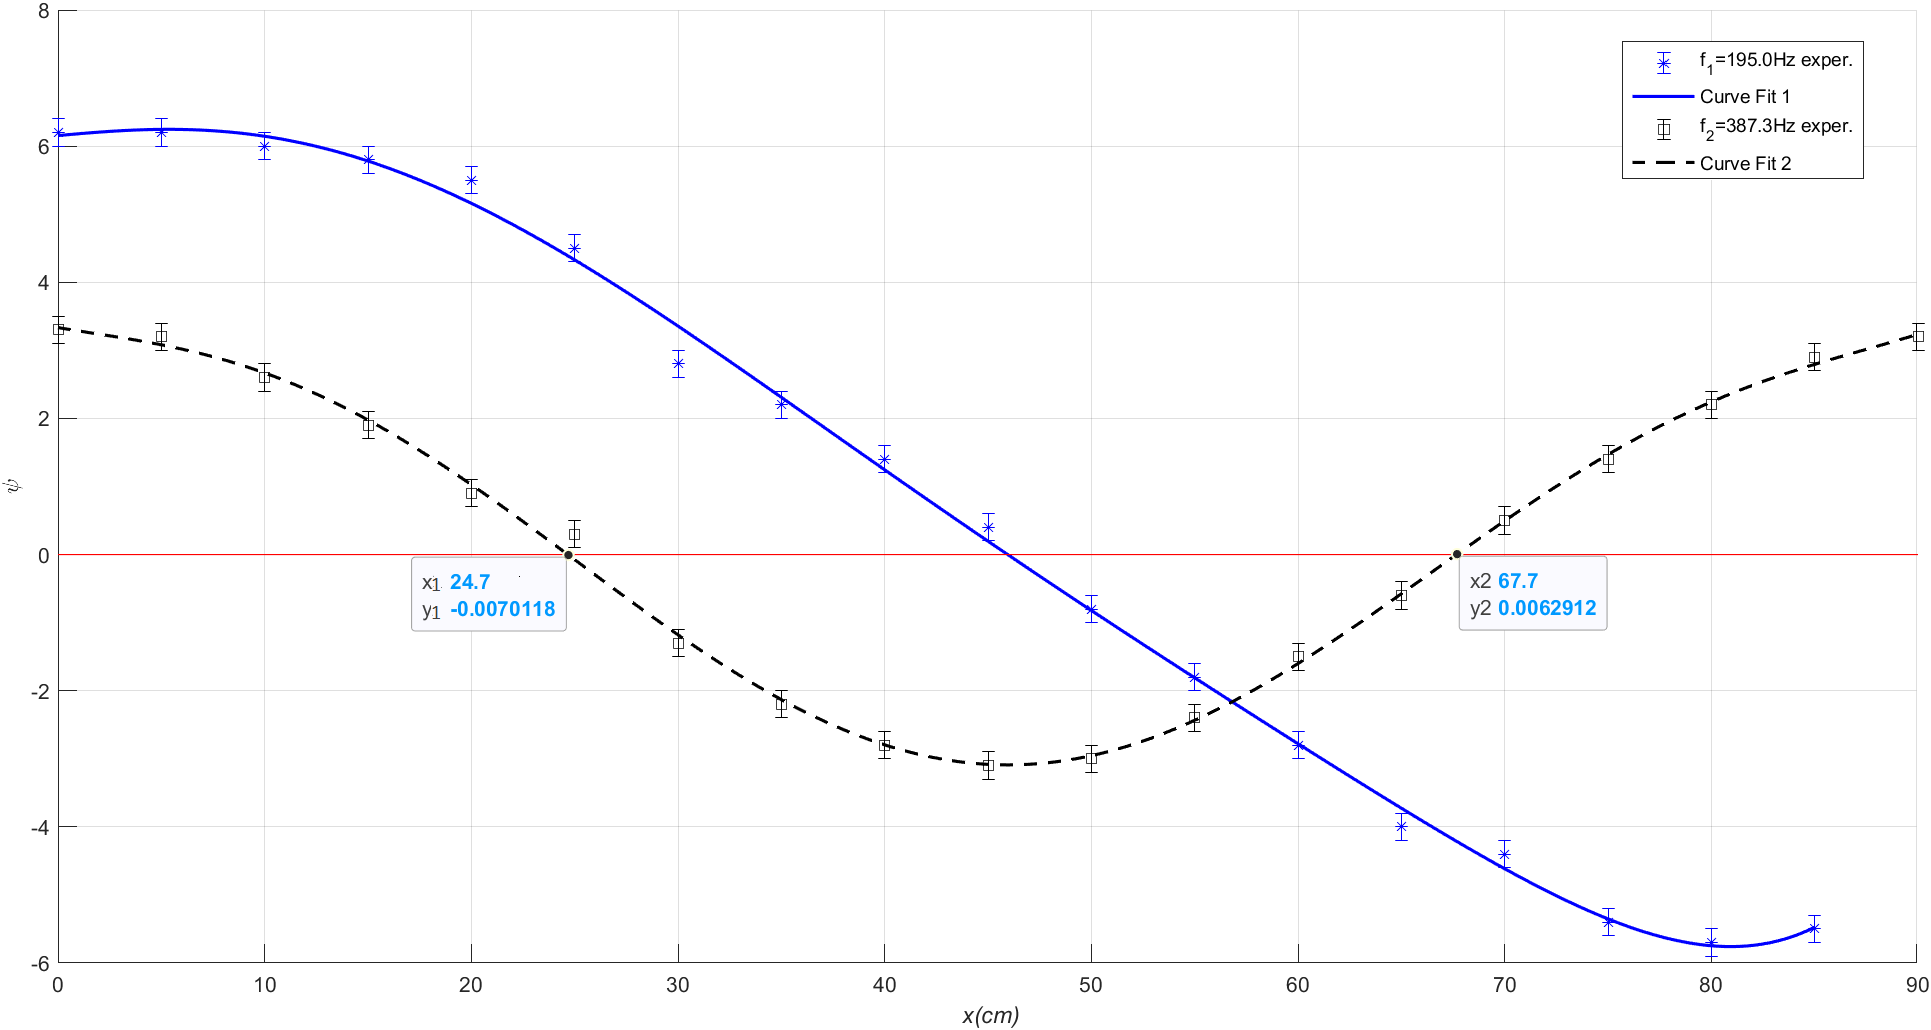
\includegraphics[scale=0.5]{plotclosed.png}
\end{figure}
 
Τώρα αφαιρούμε τον ανακλαστήρα από το δεξί άρκο και επαναλαμβάνουμε την ίδια διαδικασία μελετώντας πλέον την δεύτερη συνοριακή συνθήκη Κλειστού-Ανοικτού άκρου. Οι πρώτες τέσσερις συχνότητες συντονισμού για τις οποίες το πλάτος πίεσης μεγιστοποιείται φαίνονται στον Πίνακα 3.\footnote{Το σφάλμα για τις πειραματικές συχνότητες είναι $0.5\%$.} 
\begin{table}
\centering 
\caption{ }
\begin{tabular}{r|r|r}
n & $f_{experimental}(Hz)$ & $f_{theoretical}(Hz)$\footnotemark \\ 
\hline\hline
1 & $108.8\pm0.5$ & $94.7 \pm0.1$  \\
3 & $295.0\pm1.5$ & $284.0\pm0.1$\\
5 & $483.1\pm2.4$ & $473.3\pm0.1$ \\
7 & $670.0\pm3.4$ & $662.6\pm0.1$
\end{tabular}
\end{table}

Ομοίως με την προηγούμενη περίπτωση θεωρητικές και πειραματικές τιμές δεν συμπίπτουν ούτε στα όρια του σφάλματός τους με την σχετική διαφορά του να είναι $\sim 1-3\%$. Οι λόγοι για την εν λόγω διαφορά είναι όμοιοι με πριν. 

Επαναλαμβάνουμε την διαδικασία για τις δύο θεμελιώδεις αρμονικές $f_1=108.8Hz, f_2=295.0Hz$ και παίρνουμε τα αποτελέσματα: 


\footnotetext{Οι θεωρητικές τιμές προκύπτουν από την σχέση (\ref{4}) συνδυάζοντάς την με την $u=\lambda f$, δηλαδή $f_n=nu/4L_a$, όπου το ακουστικό μήκος είναι $L_a= L + 0.63 r = 91.008\simeq91.0cm$. To σφάλμα προκύπτει από διάδοση του σφάλματος της ταχύτητας $\delta f_n=n\delta u/4L_a$ και στρογγυλοποιώντας τα όλα είναι προκύπτουν $0.1Hz$.}

\begin{table}[h!]
\centering 
\caption{Μετρήσεις με άκρα Κλειστό-Ανοικτό}
\begin{tabular}{r|r|r}
x & $\overbrace{\psi_1(\pm 0.2)}^{f_1=108.8Hz}$ & $\overbrace{\psi_2 (\pm0.2)}^{f_2=295.0Hz}$ \\ 
\hline\hline
0&3.9&3.4\\ 
5&4.1&3.6\\
10&4.2&3.4\\
15&4.4&2.9\\
20&4.2&2.2\\
25&4.0&1.4\\
30&3.9&0.6\\
35&3.6&-0.5\\
40&3.3&-1.4\\
45&3.2&-2.0\\
50&2.9&-2.8\\
55&2.6&-3.2\\
60&2.3&-3.5\\
65&2.0&-3.5\\
70&1.6&-3.2\\
75&1.2&-2.6\\
80&0.9&-1.8\\
85&0.5&-1.0\\
90&0.1&-0.2
\end{tabular}
\end{table}
Οι πειραματικές καμπύλες για την περίπτωση ανοικτού-κλειστού άκρου και για τις 2 πρώτες συχνότητες συντονισμού φαίνονται στην Εικόνα 2.

\begin{figure}[h!]
%\centering 
\caption{ }
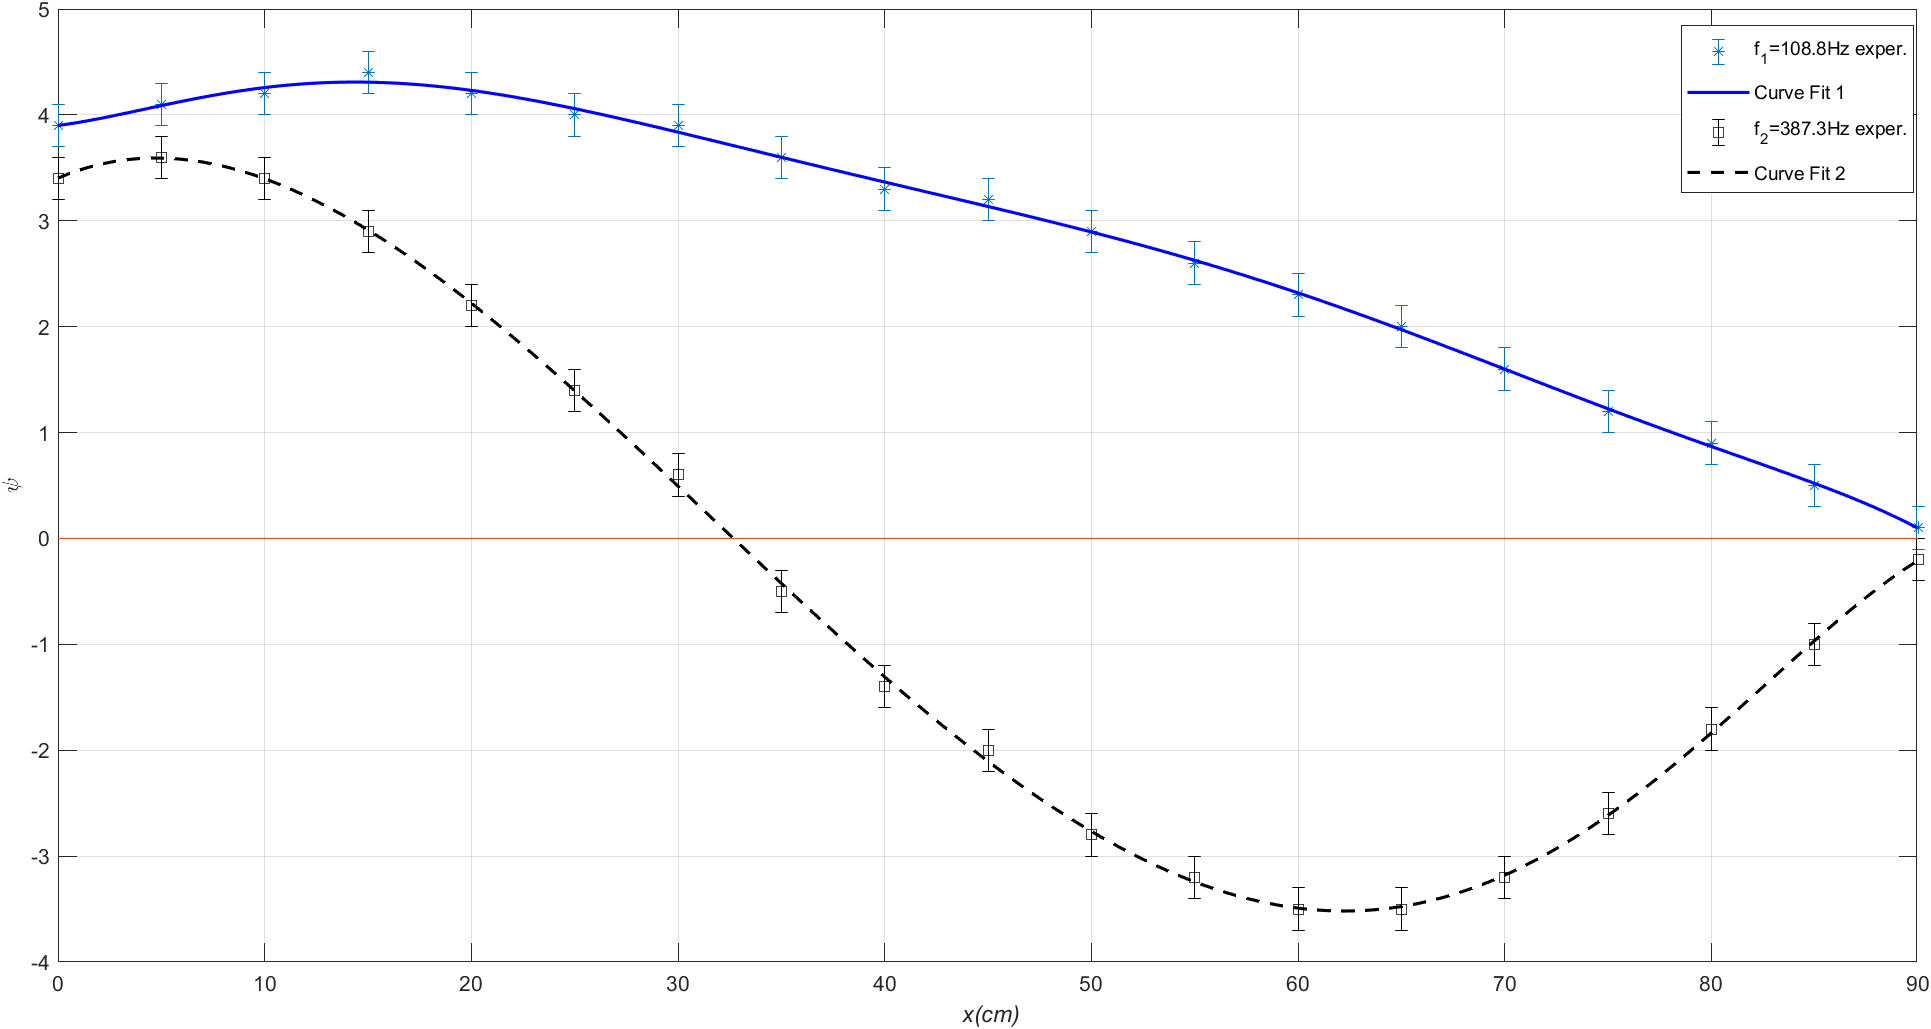
\includegraphics[scale=0.5]{plotopen.png}
\end{figure}
 
Για τον υπολογισμό της ταχύτητας του ήχου θα επιλέξω να δουλέψω με μία απ' τις πρώτες δύο καμπύλες καθώς οι αντίστοιχες μετρήσεις δεν αυξάνουν μετά την πρώτη μέτρηση όπως συμβαίνει με τις δύο τελευταίες. Πίο συγκεκριμένα, επιλέγω αυτή για $f_2=387.3Hz$ για άκρα κλειστό-κλειστό διότι η πρώτη έχει σημεία που απέχουν πολύ από την καμπύλη και επίσης δεν έχουμε την τελευταία μέτρηση.

%Για τον υπολογισμό της ταχύτητας του ήχου θα επιλέξω να δουλέψω με μία απ' τις πρώτες δύο καμπύλες, καθώς οι πρώτες μετρήσεις για τις δύο δεύτερες δίνουν μεγαλύτερο πλάτος αντί για μικρότερο. Πιό συγκεκριμένα, επιλέγω την καμπύλη για $f_2=387.3Hz$ για άκρα Κλειστό-Κλειστό διότι η άλλη έχει σημεία που απέχουν πολύ (εκτός ορίου σφάλματος) από την καμπύλη και επίσης δεν έχουμε την τελευταία μέτρηση.

Όπως έχει αναφερθεί, η απόσταση μεταξύ διαδιχικών κοιλιών ή δεσμών μετατόπισης άρα και πίεσης είναι $\lambda /2$. Επομένως, από την καμπύλη που επιλέχθηκε έχουμε: 
\begin{align*}
\lambda_{KK2,exp.} = 2(x_2-x_1)\pm\delta\lambda_{KK2,exp.} = 2(67.7-24.7)\pm0.3 \Rightarrow \\ 
\boxed{\lambda_{KK2,exp.} = (86.0\pm0.3)cm}
\end{align*}
όπου το σφάλμα προκύπτει από διάδοση: 
\begin{align*}
\delta (\lambda_{KK2,exp.}/2) &= \sqrt{\left( \pdv{(x_2-x_1)}{x_1}\delta x_1 \right)^2 + \left( \pdv{(x_2-x_1)}{x_2}\delta x_2 \right)^2  } \xRightarrow{\delta x_1 = \delta x_2} \\ 
\delta\lambda_{KK2,exp.} &= 2\sqrt{2}\delta x_2 =2\sqrt{2}\cdot 0.1\Rightarrow \delta\lambda_{KK2,exp.} = 0.2828 \simeq 0.3 cm
\end{align*}

 Τώρα από την σχέση $u=\lambda_{KK2,exp}f_2\pm\delta u$ θα προκύψει και η ταχύτητα του ηχητικού κύματος στον αέρα: 
 \begin{align*}
 \boxed{u = (333.1\pm 2.0) m /s }
 \end{align*}
 Για το σφάλμα έχουμε: 
 \begin{align*}
 	\delta u &= \sqrt{\left( \pdv{u}{\lambda_{KK2,exp.}}\delta\lambda_{KK2,exp.} \right)^2 + \left( \pdv{u}{f_2}\delta f_{2} \right)^2 }\Rightarrow \\ 
 	&= \sqrt{(f_2\delta\lambda_{KK2,exp.})^2 + (\lambda_{KK2,exp.}f_2)^2} = 2.0005\simeq 2.0 m/s
 \end{align*}
 
 Παρατηρώ ότι η παραπάνω ταχύτητα δεν συμπίπτει με την θεωρητική όπως υπολογίστηκε από την σχέση (\ref{5}) ούτε στα πλαίσια των σφαλμάτων και απέχει από αυτή $\sim 3.5\%$ της τιμής της. 
 
 \subsubsection*{2ο Μέρος: Μέθοδος radar}
 Σε αυτό το μέρος ο στόχος είναι η μέτρηση της ταχύτητας του ήχου με τη μέθοδο radar. Ρυθμίζουμε την γεννήτρια ώστε να παράγει ορθογώνιους παλμούς πλάτους 5V και συχνότητας $f=10Hz$, τοποθετούμε το μικρόφωνο στην αρχή του σωλήνα, ενώ ταυτόχρονα κλείνουμε το δεξί άκρο με τον ανακλαστήρα.
 
 Η γεννήτρια εξαναγκάζει την μεμβράνη του μεγαφώνου να κινείται προς τα αριστερά 10 φορές το δευτερόλεπτο. Κατά την κίνησή της προς τα αριστερά παράγεται ένας κρουστικός παλμός αραίωσης ενώ μετά από 0.05s όταν η μεμβράνη επιστρέφει στην αρχική της θέση παράγεται κρουστικός παλμός πύκνωσης. 
% Οι παλμοί έπειτα από την ανάκλασή τους συμβάλλουν και ταυτόχρονα ο κάθε ένας ανακλάται διαρκώς από τα άκρα του σωλήνα με αποτέλεσμα να φθίνει εκθετικά πλάτος του λόγω απωλειών. Στο κανάλι του παλμογράφου μπορούμε να διακρίνουμε παλμούς που έχουν υποστεί εως και 10 ανακλάσεις.
Οι παλμοί ανακλώνται διαρκώς στα άκρα του σωλήνα και ταυτόχρονα συμβάλλουν μεταξύ τους. Κατά την ανάκλαση υπάρχουν απώλειες με αποτέλεσμα την εκθετική μείωση του πλάτους.
Στον παλμογράφο μπορούμε να διακρίνουμε παλμούς που έχουν υποστεί εως και 10 ανακλάσεις
 
 Από την οπτική εικόνα που παρατηρούμε στο κανάλι του μικροφώνου μπορούμε να δούμε τον χρόνο που απαιτείται για να ταξιδέψουν 9 μπρος-πίσω κατά μήκος του σωληνα. Η κάθε κορυφή πίεσης που βλέπουμε αντιστοιχεί σε μία διαδρομή, εκτός από την πρώτη που πρόκειται για την απευθείας ανίχνευση του κύματος από το μεγάφωνο. Βλέπουμε 10 κορυφές άρα 9 διαδρομές. Ωστόσο, επειδή η τελευταία κορυφή είναι πολύ αμυδρή μετράμε τον χρόνο για 9 κορυφές δηλαδή 8 διαδρομές:
 \begin{align*}
 t_8=(8.4\pm0.2)5m s \Rightarrow t_8 = (42.0\pm1.0)m s
  \end{align*}
  Άρα η ταχύτητα του ήχου προκύπτει 
  \begin{align*}
  \boxed{u = (342.9\pm8.2) m/s} \footnotemark
  \end{align*}
  \footnotetext{Η ταχύτητα προκύπτει: $u=8 (2L)/t_8 = 342.9m/s$  και το σφάλμα της $\delta u=\sqrt{\left( \pdv{u}{L}\delta L \right)^2+\left( \pdv{u}{t_8}\delta t_8 \right)^2}=16\sqrt{(\delta L/t_8 )^2 + (L\delta t_8 /t_8^2)^2} = 8.1721\simeq8.2m/s$}.
  
  Εμφανώς αυτή η μέθοδος δίνει αποτέλεσμα που συμπίπτει στα όρια του σφάλματος με την θεωρητική τιμή της σχέσης (\ref{5}) και απέχει από αυτήν $\sim0.5\%$ έναντι του $\sim 3.5\%$ που απέχει η τιμή που βρέθηκε από την προηγούμενη μέθοδο.
  
  Τέλος, πρέπει να σημειωθεί το γεγονός ότι οι πρώτες 10 κορυφές που είναι εμφανείς βρίσκονται στα αρνητικά, που σημαίνει ότι το μικρόφωνο ανιχνεύει αραιώματα, ενώ μετά τους πρώτους δέκα οι κορυφές είναι θετικές, άρα ανιχνεύονται πυκνώματα. 
  Ωστόσο, αν αφαιρέσουμε τον ανακλαστήρα παρατηρούμε πως οι κορυφές εναλάσσονται και είναι μία θετική μία αρνητική. Η ανίχνευση των κορυφών φανερώνει ότι ο ηχητικός παλμός ανακλάται στο ανοικτό άκρο διότι η μετάβαση στο εξωτερικό του σωλήνα του επιβάλλει την διάδοσή του ως σφαιρικό κύμα, άρα η έντασή του μειώνεται με το τετράγωνο της απόστασης. Έτσι, θεωρούμε ότι μεταβαίνει από ένα μέσο μικρής εμπέδησης σε ένα μεγαλύτερης και γι' αυτό συναντάμε το φαινόμενο της ανάκλασης.
   Η ένταση παίρνει πολύ μικρή τιμή περίπου σε απόσταση 0.63r εκτός του σωλήνα, όπου και θεωρούμε πως γίνεται η ανάκλαση. Ακόμη η εναλλαγή του προσήμου των κορυφών του σήματος ανίχνευσης δηλώνει την μετατροπή πυκνώματος σε αραίωμα και αντιστρόφως κατά την διαδικασία την ανάκλασης, δηλαδή έχουμε αρνητικό συντελεστή ανάκλασης για την πίεση ($R_p=-1$).
\section*{Συμπεράσματα}
Στο πρώτο μέρος του πειράματος πήραμε την αναμενόμενη μορφή των καμπυλών κατανομής της πίεσης. Ωστόσο η εκτίμηση της ταχύτητας του ήχου με την εν λόγω μέθοδο δεν ήταν ικανοποιητική, καθως απείχε από την θεωρητική $\sim 5\%3.$ της τιμής της. Αντίθετα, στο δέυτερο μέρος ο υπολογισμός της ταχύτητας του ήχου ηταν εξαιρετικά ακριβής προσεγγίζοντας την θεωρητική τιμή με διαφορά $\sim 50.5\%$. 

Η διαφορά στην ακρίβεια του υπολογισμού εικάζω ότι προέρχεται από το γεγονός ότι το πρώτο μέρος είχε περισσότερα πειραματικά βήματα, επομένως ίσως να υπήρχαν συστηματικά σφάλματα που έχουν αγνοηθεί. Μερικά από έχουν ήδη αναφερθεί και είναι η υψηλή ευαισθησία του ποτενσιομέτρου επιλογής συχνότητας και η μη ακριβής τοποθέτηση του σήματος στους άξονες του παλμογράφου.


\end{document}